\documentclass[12pt, letterpaper]{article}
\usepackage{amsmath}
\usepackage{enumitem}
\usepackage{graphicx}



\title{Assignment 1 \\ CS 591B 3D COMPUTER VISION}
\author{Ryan Watson }
\date{Due: $26^{th}$ September 2017}
 
\begin{document}
 
\begin{titlepage}
\clearpage\maketitle
\thispagestyle{empty}
\end{titlepage}

%-----------------------------------------------------------------------------------------------%
%-----------------------------------------------------------------------------------------------%

\noindent {\bf{Question 1)}} \hspace{0.4cm} A certain object in front of a camera with a focal length of 16 millimeters is well focused when the focal distance is 16.4 millimeters.
 
\begin{enumerate}[label=\Alph*]
 	\item How far is the object from the camera?
 	\item If the distance of the object to the camera is cut in half, where does it focus now?
\end{enumerate} 

{\bf{ Answer \\}}
\indent {\bf{ A: \\}} 
\indent From the thin lens equation, we know that 
\begin{equation*}
\frac{1}{f} = \frac{1}{z} - \frac{1}{Z} \quad \rightarrow Z = \frac{zf}{f-z}.
\end{equation*}
\indent The above relation tells us that the object is {\bf{656 millimeters}} away.

\vspace{0.2cm}
{\bf{B: \\}}
\indent Again, using the thin lens equation, we can get the relation, 
\begin{equation*}
\frac{1}{f} = \frac{1}{z} - \frac{1}{Z} \quad \rightarrow f = \frac{1}{\frac{1}{z} - \frac{1}{Z}}.
\end{equation*}
\indent The above relation tells us that the new focus is {\bf{17.3 millimeters}}.


%-----------------------------------------------------------------------------------------------%
%-----------------------------------------------------------------------------------------------%

\vspace{1.5cm}
\noindent {\bf{Question 2)}} \hspace{0.4cm} A camera is coincident with the world coordinate system as shown in the figure below. The image plane of the camera is at z = 1. A solid cube of side length 10
is centered at (0, 0,−40). Where in the camera's image plane are the visible corners of the cube
imaged?

\begin{center}
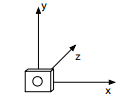
\includegraphics[scale=1]{figs/cam_model.png}
\end{center}

{\bf{ Answer \\}}

From the pinhole projection model, we are provide the transformation below

 \[
      f(P)=\left\{
                \begin{array}{ll}
                  x = d \frac{X}{Z} \\
                  y = d \frac{Y}{Z} . \\
                \end{array}
              \right.
  \]
  
\indent To utilize the above mentioned equation, the points in the world coordinate system must first be defined.

$$
P_1 =  \begin{bmatrix} 5\\5\\-35 \end{bmatrix}, \quad P_2 =  \begin{bmatrix} -5\\5\\-35 \end{bmatrix}, \quad P_3 =  \begin{bmatrix} -5\\-5\\-35 \end{bmatrix}, \quad P_4 =  \begin{bmatrix} 5\\-5\\-35 \end{bmatrix}.
$$

Now, we can project all of the vectors as shown below 

$$
f(P_1) =  \begin{bmatrix} 0.14\\0.14 \end{bmatrix}, \quad f(P_2) =  \begin{bmatrix} -0.14\\0.14 \end{bmatrix}, \quad f(P_3) =  \begin{bmatrix} -0.14\\-0.14 \end{bmatrix}, \quad f(P_4) =  \begin{bmatrix} 0.14\\-0.14 \end{bmatrix}.
$$

%-----------------------------------------------------------------------------------------------%
%-----------------------------------------------------------------------------------------------%

\vspace{1.5cm}
\noindent {\bf{Question 3)}} \hspace{0.4cm} Given the following rigid transformation,

$$ 
T_{O}^{O'} = 
\begin{bmatrix} 
R & t \\
0^{T} & 1 
\end{bmatrix}
$$

\indent derive the inverse transformation $T_{O'}^{O}$ . It must be written as a function of the rotation matrix $R \in \mathbf{R}^{3x3}$ and the translation vector $t \in \mathbf{R}^{1x3}$. \\

{\bf{ Answer \\}}

\indent We can start by noting that $ T^{O'}_{O} T^{O}_{O'} = I $ $ \iff $ $ T^{O}_{O'} = (T^{O'}_{O} )^{-1} $. Now, we can assume a generic form for the inverse matrix, $T_{O'}^{O} = \begin{bmatrix}  A & B \\ C & D  \end{bmatrix}$. This gives us a system of constraints, 

\[
	\left\{
           \begin{array}{ll}
                  RA +tC = I\\
                  RB + tD = 0\\
                  C = 0 \\ 
                  D = I \\ 
                \end{array}
              \right.
  \]

\indent Solving for the coefficients, A,B,C,D, we find that the inverse of the transformation is

$$ T_{O'}^{O} = 
\begin{bmatrix} 
R^{T} & -R^{T}t \\
0^{T} & 1 
\end{bmatrix}
$$


%-----------------------------------------------------------------------------------------------%
%-----------------------------------------------------------------------------------------------%

\vspace{1.5cm}
\noindent {\bf{Question 4)}} \hspace{0.4cm} Given the camera array that is shown in the figure below, find the algebraic expression to calculate the transformation $T^{C2}_{C1}$ as a function of the camera poses $T^{C1}_{W}$ and $T^{C2}_{W}$ for camera $C_{1}$ and $C_{2}$, respectively


\begin{center}
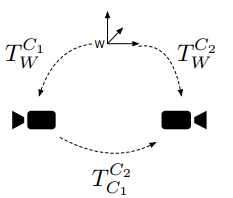
\includegraphics[scale=0.7]{figs/rigid_trans.png}
\end{center}

{\bf{ Answer \\}}

\indent The transformation between any two coordinate frames can be calculated by utilizing the commonly reference relation, 

$$ T_{a}^{b} = T^{b}_{d}T^{d}_{a}. $$

\indent Thus, the transformation, $T^{C2}_{C1}$, can be calculated as 

$$ T^{C2}_{C1} = T^{C2}_{W} ( T^{W}_{C1} ), $$

\indent where $T^{W}_{C1} = (T^{C1}_{W})^{T}$ because $T^{C1}_{W}$ is an orthogonal matrix.


%-----------------------------------------------------------------------------------------------%
%-----------------------------------------------------------------------------------------------%

\vspace{1.5cm}
\noindent {\bf{Question 5)}} \hspace{0.4cm} Two cameras are co-aligned along the x-axis and are 20 units
apart of each other. Camera C1 is centered at the origin of the world coordinate system. If both
cameras have the same calibration matrix:

\begin{center}
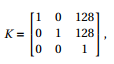
\includegraphics[scale=0.7]{figs/camera_cal.png}
\end{center}

what are the pixel coordinates of the four points (A - D) on the checkerboard in both cameras?
See figure below.

\begin{center}
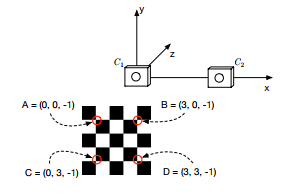
\includegraphics[scale=0.7]{figs/checker_board.png}
\end{center}

{\bf{ Answer \\}}

\indent The points in the image plane can be calculated using the relation provided below,

$$ p = \frac{1}{Z}KP $$

\indent {\bf{Camera C1}} 

\indent $ A_{C1} = \frac{1}{Z}KP = \frac{1}{1}\begin{bmatrix}  1&0&128 \\ 0&1&128 \\ 0&0&1  \end{bmatrix} \begin{bmatrix} 0\\0\\-1 \end{bmatrix} = \begin{bmatrix} 128\\128 \end{bmatrix} $

\vspace{0.4cm}
\indent $ B_{C1} = \frac{1}{Z}KP = \frac{1}{1}\begin{bmatrix}  1&0&128 \\ 0&1&128 \\ 0&0&1  \end{bmatrix} \begin{bmatrix} 3\\0\\-1 \end{bmatrix} = \begin{bmatrix} 125\\128 \end{bmatrix} $

\vspace{0.4cm}
\indent $ C_{C1} = \frac{1}{Z}KP = \frac{1}{1}\begin{bmatrix}  1&0&128 \\ 0&1&128 \\ 0&0&1  \end{bmatrix} \begin{bmatrix} 0\\3\\-1 \end{bmatrix} = \begin{bmatrix} 128\\122 \end{bmatrix} $

\vspace{0.4cm}
\indent $ D_{C1} = \frac{1}{Z}KP = \frac{1}{1}\begin{bmatrix}  1&0&128 \\ 0&1&128 \\ 0&0&1  \end{bmatrix} \begin{bmatrix} 3\\3\\-1 \end{bmatrix} = \begin{bmatrix} 125\\125 \end{bmatrix} $

\vspace{0.6cm}
\indent {\bf{Camera C2}} 

For camera, C2, we must augment the above equation to translate the points to be coincident with C1. 

\indent $ A_{C1} = \frac{1}{Z}K(P+t) = \frac{1}{1}\begin{bmatrix}  1&0&128 \\ 0&1&128 \\ 0&0&1  \end{bmatrix} ( \begin{bmatrix} 0\\0\\-1 \end{bmatrix}+\begin{bmatrix} 20\\0\\0 \end{bmatrix}
) = \begin{bmatrix} 108\\128 \end{bmatrix} $

\vspace{0.4cm}
\indent $ B_{C1} = \frac{1}{Z}K(P+t) = \frac{1}{1}\begin{bmatrix}  1&0&128 \\ 0&1&128 \\ 0&0&1  \end{bmatrix} (\begin{bmatrix} 3\\0\\-1 \end{bmatrix}+\begin{bmatrix} 20\\0\\0 \end{bmatrix}
) = \begin{bmatrix} 105\\128 \end{bmatrix} $

\vspace{0.4cm}
\indent $ C_{C1} = \frac{1}{Z}K(P+t) = \frac{1}{1}\begin{bmatrix}  1&0&128 \\ 0&1&128 \\ 0&0&1  \end{bmatrix} (\begin{bmatrix} 0\\3\\-1 \end{bmatrix} + \begin{bmatrix} 20\\0\\0 \end{bmatrix}
)  = \begin{bmatrix} 108\\125 \end{bmatrix} $

\vspace{0.4cm}
\indent $ D_{C1} = \frac{1}{Z}K(P+t) = \frac{1}{1}\begin{bmatrix}  1&0&128 \\ 0&1&128 \\ 0&0&1  \end{bmatrix} ( \begin{bmatrix} 3\\3\\-1 \end{bmatrix} + \begin{bmatrix} 20\\0\\0 \end{bmatrix}
 ) = \begin{bmatrix} 105\\105 \end{bmatrix} $


%-----------------------------------------------------------------------------------------------%
%-----------------------------------------------------------------------------------------------%

\vspace{1.5cm}
\noindent {\bf{Question 6)}} \hspace{0.4cm} Find the calibration parameters (intrinsic/calibration matrix, all extrinsic parameters, and radial distortion coefficients) of the camera used to take images of the checkerboard. The checkerboard images can be downloaded from e-campus. Only report the intrinsic
calibration parameters.

{\bf{ Answer \\}} Using the Matlab Camera Calibration Toolbox -- specifically, the ${\it{calib\_gui}}$ was utilized -- we can find the camera calibration parameters. 

First, we will correct for the radial distortion.

$$ x = x(1+k_1r^2 + k_2r^4 + k_3r^6) $$

$$ y = y(1 + k_1r^2 + k_2r^4 + k_3r^6) $$ 

Next, we can correct for the tangential distortion. 

$$ x = x + [ 2p_1xy + p_2(r^2+2x^2)] $$ 

$$ y = y + [p1(r^2+2y^2)+2p_2xy] $$  

Where our distortion vector is calculated using the Camera Calibration Toolbox 
$$
D = \begin{bmatrix} k_1\\k_2\\p_1\\p_2\\k_3  \end{bmatrix} = \begin{bmatrix} 0.16707\\-0.06990\\-0.00444\\0.00747\\0.00000  \end{bmatrix} $$

Finally, our camera calibration matrix is defined as,

$$ 
K = \begin{bmatrix}  \alpha&-\alpha cot \theta & u_o \\ 0& \frac{\beta}{sin \theta} & v_o \\ 0&0&1  \end{bmatrix} = \begin{bmatrix}  3830.77480 & 0 & 2166.40247 \\ 0& 3827.36501 & 1163.82736 \\ 0&0&1  \end{bmatrix}
$$
\indent 

\end{document}